\chapter{Hyperbolic representations }\label{chap:hyperbolics}

What is the position of Gyrovector formalism, Einstein midpoints, and, often
set-free, hyperbolic geometry as relative to the framework of differential
geometry?

\citet{beardonMindaHyp} do a good job at introducing different models of
Hyperbolic geometry and their metrics, but allows certain amount of
implicitness -- it is sometimes not clear where their Mathematics is
internalized in, and what exactly are types of objects they operate with. We'd
like to see a similar treatment of the subject but consistent with the language
of Frederic Schuller's lectures, which we chose as a reference.

\citet{lavenda2008relativity} discusses hyperbolic rigid motions
in connection to velocities of special relativity.
Somewhat similar is~\citet{barrett2011hyperbolic} (with hand-drawn
visualization -- nice!).

\citet{snyder2009isometries} carries out computations for upper half-plane
model -- useful after half-plane model is introduced (it isn't one most
intuitive to start with).

\citet{droyster} apparently taught a nice course on the subject sometime, and
provides a number of great links.

\citet{ungarDiffGeom} connects Ungar's Gyrovector formalism with related
concepts in differential geometry, but assumes an ``intuitive understanding''
of the subject, rather than explicit descriptions. For instance, the author
talks about ``differentials'' \( \Delta s = (v + \Delta v) - v \) rather than
tangent vectors\footnote{And one should acknowledge that many physicists tend
to understand these not even as ``infinitesimals'', but as actual ``small
numbers''}. In other words, we're not satisfied by their description because of
\emph{dynamic typing}. One more nuisance with their approach is that it begins
with rather overwhelming and abstract axiomatic description of Gyrovector
spaces and groups, rather than with description of hyperbolic motions followed
by summarization of their \emph{properties}.  In the first case we get a huge
number of mutually redundant \emph{axioms} in the premises of the theory, and
these axioms aren't something people have thoroughly discussed and learned to
accept as foundations. In the second case, these ``axioms'' are \emph{useful
consequences} of something we already live with.

\section{An outline of a possible introduction of hyperbolic geometry}

We first introduce the Hyperbolic space as the upper sheet of the Hyperboloid in
a Minkowski flat space -- the \( \mathbb{R}^{n+1} \) endowed with Minkowski
pseudo-inner product and trivial metric manifold structure.
The Hyperboloid inherits the local metric from ambient Minkowski space via the
pull-back under trivial (identity) embedding -- the inherited metric is
actually a Riemannian (positively-definite) one, although we skip demonstration
of this fact.
The upper-sheet can be projected onto Poincar\'e ball model -- the unit ball in
\( \mathbb{R}^n \), and further to upper-halfspace
\( \{x\in\mathbb{R}^n\left|x_n > 0 \right. \} \), always inheriting the local
metric using pull-back under inverse of projection.  Until this point, we only
discuss underlying sets and local differential properties, such as local
metric. To evaluate synthetic properties of the Hyperbolic space, e.g. to
compute distances between points, it is often convenient to switch between the
available models arbitrarily -- they are isometric by construction, while
different tasks are easier accomplished in different models.

For instance, in the upper half-plane the local metric becomes \(
\frac{y^2}(\operatorname{d}\mathrm{x}^2 + \operatorname{d}\mathrm{y}^2) \) and
it becomes obvious that for two points on the same vertical line the geodesic
curve that connects them is the segment of vertical line.  It is also
straigtforward to compute the length integral of that curve and obtain \( \ln
y_1 - \ln y_0 \) for points \( (x, y_1) \), \( (x, y_0) \), with \( y_1 \geq
y_0 \). Computation of distances between arbitrary points becomes possible,
when one discovers an \emph{isometric} self-map that puts any two points onto
same vertical (in fact one can move any \emph{triple} to any desired places in
the half-plane).

An important observation is that mappings between all the mentioned models of
Hyperbolic geometry are realized by so-called \emph{inversions} in spheres and
planes. Moreover, \emph{all} isometric self-maps of introduced hyperbolic
spaces are realized by finite combinations of such
inversions~\cite{beardonMindaHyp,beardonGeometryDiscrete,visualComplexAn}.
Finite compositions
of inversions are called \emph{M\"obius transforms} and they are key to
analysis of hyperbolic motions, i.e. to the discussion of geodesics and
exponential maps in hyperbolic model spaces. Ungar's gyro-operations
can be seen as a convenient language for discussion of isometric M\"obius
transformations of Poincar\'e ball.  The fact that (compositions of) inversions in planes and
spheres describe all possible isometries is fundamental. For example, while we
generally like \emph{balls} and deem them relatively simple constructions, it
would feel \emph{unnatural} to propose a half-plane as the first model of
Hyperbolic geometry. One could think: ``there must be an intrinsic reason we
got to cut the other half off''. Inversions turning spheres into planes is
exactly that intrinsic reason.

Studying isometries one should conclude about geodesics, exponential maps, and
parallel transportation in hyperbolic model spaces. Connections to Ungar's
gyro-formalism could be outlined. At this point one must be able to implement
the basic Riemannian gradient descent on these spaces.

Finally, we'd like to evaluate various measures of curvature in these spaces.
Alack we couldn't do that in time.

\section{Hyperboloid and Poincar\'e disk models} \label{sec:poincareBall}

It seems to be a reasonably motivated to introduce a hyperbolic metric by
starting with the Hyperboloid model. For instance, we'll take on intuition
of~\cite{thurstonThree} and set out to construct a ``sphere'' of constant
negative curvature \( \frac{1}{r^2} = -1 \), i.e. ``of imaginary radius \( r=i
\)''.

Consider the Lorentz (Minkowski) space -- the \( (\mathbb{R}^{n+1}, Q) \),
consisting of points \( (x_1, \ldots, x_n, t) \) (conveniently denoted \( (x,
t) \)), endowed with a non-degenerate symmetric bilinear form
\[ Q((x, t), (x', t')) = \sum_{k=1}^n x_k x_k' - tt', \]
and corresponding pseudo-Riemannian metric \[ g_H = \operatorname{d}\mathrm{x}_1^2 +
\cdots + \operatorname{d}\mathrm{x}_n^2 - \operatorname{d}\mathrm{t}^2, \]
where \( \operatorname{d}\mathrm{x}_j \) is the chart-induced basis covector, as
introduced in previous appendix (we use straight characters \( \mathrm{x}_i \),
as opposed to \( x_i \) to denote the chart component \emph{functions}; in this
case chart is the identity and chart components are projections).

The underlying set of our model space is the upper sheet of the \(n\)-dimensional
Hyperboloid:

\begin{align*}
H &= \left\{ (x, t) \in \mathbb{R}^{n+1} \left| Q((x,t), (x,t)) = -1,~ t>0 \right.\right\}\\
&= \left\{ (x, t) \in \mathbb{R}^{n+1} \left| \sum_{k=1}^n x_k^2 - t^2 = -1,~t>0 \right.\right\}.
\end{align*}

\begin{wrapfigure}{r}{.25\textwidth}
    \center
    \caption{Tiling of the Poincar\'e Disk by~\citet{bulatovConformal}. The lines
    are geodesic curves}
    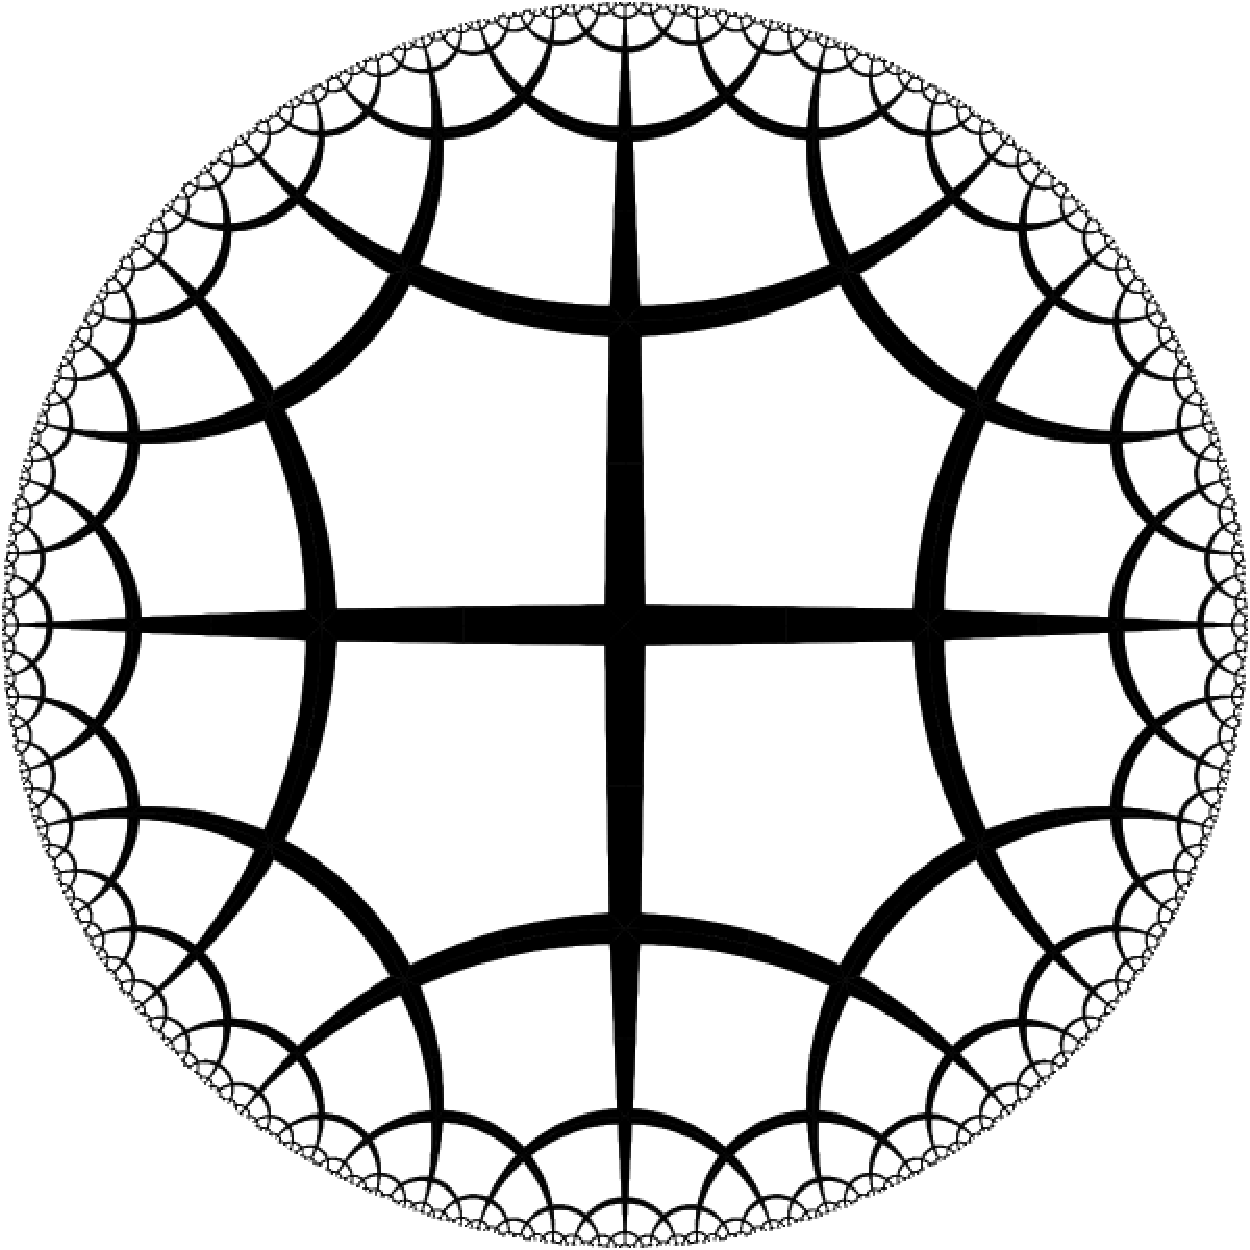
\includegraphics[width=.8 \linewidth]{art/tiling-disk.pdf}
\end{wrapfigure}

The upper-sheet is a metric manifold, with global chart
\( (x, x_{n+1}) \mapsto x \) and its inverse
\( x \mapsto (x, \sqrt{1 + \|x\|_2^2}) \). The local metric is induced from
ambient Minkowski space. This
pull-back metric is a Riemannian (positive-definite) metric. However, instead
of investigating this metric on the Hyperboloid, we will straight away consider
the Stereographic projection that maps upper-sheet onto the \emph{Poincar\'e
ball}
\( \mathcal{P} = \{ p\in\mathbb{R}^n\left|~\|p\|_2^2 \leq 1\right.\}. \)
This map is realized as follows: a point \( (x, t) \) on the upper-sheet is
projected onto the horizontal plane \( \{ (y, 0) \left| y\in
\mathbb{R}^{n}\right. \} \) with the center of projection at the vertex of the
lower-sheet, i.e. \( (0, -1) \). One can easily derive that the projection is \(
(x, t) \mapsto \frac{1}{1+t}x: H\to\mathcal{P} \), and has the inverse \(
\phi:\mathcal{P}\to H, \)

\[ \phi(p) = (\frac{2p}{1 - \|p\|_2^2},~\frac{1+\|p\|_2^2}{1-\|p\|_2^2}). \]

The Poincar\'e ball has a very natural global chart -- the identity map \(
\mathrm{p}=p\mapsto p \), which induces a convenient basis of partial
derivatives,
\( \operatorname{id}_*\partial_i\simeq\partial_i,~i=\overline{1,n}, \) in the
tangent bundle \( \mathcal{T}\mathcal{P} \). The projection inverse \( \phi \)
allows to pull-back the Minkowski metric inherited by upper-sheet onto
Poincar\'e disk: \[ (\operatorname{id}_{H\to(\mathbb{R}^{n+1},~g_H)}\circ~
\phi)^* g_H = \phi^*g_H. \]
It's useful to describe this metric in chart-induced
coordinates. Specifically, we need to compute
\[ g_H(\phi_* \partial_i,~\phi_* \partial_j). \]

A tangent vector \( \phi_*\partial_i \in \mathcal{T}\mathbb{R}^{n+1} \) is
naturally described by its action on a scalar function \(
f:\mathbb{R}^{n+1}\to\mathbb{R} \), so
\begin{align*}
(\phi_* \left.\partial_i\right|_p)f &= \left.\partial_i\right|_p(f\circ \phi)\\
&= \sum_{k=1}^{n+1} (\left.\partial_k\right|_{\phi(p)} f) (\left.\partial_i\right|_p \phi_k)\\
&= \left(\sum_{k=1}^{n+1} (\partial_i \phi_k)(p) \cdot
\left.\partial_k\right|_{\phi(p)}\right) f,
\end{align*}
where we, slightly abusing notation, treat partial derivatives as
``polymorphic'', so that the ``type'' of each instance is inferred from types
of their arguments (\( f \) or \( \phi_k \)).
Further, the coefficients of basis vectors
\begin{align*}
(\partial_i\phi_k)(p)
&= \frac{2p_i}{(1-\|p\|_2^2)^2} \sum_{k=1}^{n+1} 2p_k \partial_k
+ \frac{2}{1 - \|p\|_2^2} \partial_i
+ \frac{2p_i}{1 - \|p\|_2^2} \left( \frac{1+\|p\|_2^2}{1-\|p\|_2^2} + 1\right) \partial_{n+1}\\
&= \frac{4p_i}{(1-\|p\|_2^2)^2} (\partial_{n+1} + \sum_{k=1}^{n+1} p_k \partial_k)
+ \frac{2}{1-\|p\|_2^2}\partial_i.
\end{align*}

Now we can compute the coefficients of the metric tensor.
First, for \( i\neq j \):
\begin{align*}
g_H(\phi_*\partial_i, \phi_*\partial_j)
= &~\frac{4p_i 4p_j}{(1 - \|p\|_2^2)^4}
     g_H(\partial_{n+1} + \sum_{k=1}^n p_k \partial_k,~
         \partial_{n+1} + \sum_{k=1}^n p_k \partial_k) \\
  &~+ \frac{4}{(1-\|p\|_2^2)^2} g_H(\partial_i,~\partial_j) \\
  &~+ \frac{8p_i}{(1 - \|p\|_2^2)^3} g_H(\partial_{n+1} + \sum_{k}\partial_k,~\partial_j) \\
  &~+ \frac{8p_j}{(1 - \|p\|_2^2)^3} g_H(\partial_i,~\partial_{n+1} + \sum_{k}\partial_k) \\
= &~(16p_ip_j)\frac{-1 + \|p\|_2^2}{(1 - \|p\|_2^2)^4} \\
  &~+ 0 \\
  &~+ \frac{8p_i}{(1 - \|p\|_2^2)^3} g_H(p_j \partial_j,~\partial_j) \\
  &~+ \frac{8p_j}{(1 - \|p\|_2^2)^3} g_H(\partial_j,~p_i \partial_i) \\
= &~0.
\end{align*}

Finally,
\begin{align*}
g_H(\phi_*\partial_i,~\phi_*\partial_i)
= &~\frac{-16 p_i^2}{(1 - \|p\|_2^2)^3} 
  + \frac{4}{(1-\|p\|_2^2)^2} 
  + \frac{16p_i^2}{(1 - \|p\|_2^2)^3} \\
= &~\frac{4}{(1 - \|p\|_2^2)^2}.
\end{align*}

Thus
\[ \left.\phi^*\right|_p g_H = \frac{4}{(1 - \|p\|_2^2)^2} \operatorname{d}\mathrm{p}^2. \]

This is the Poincar\'e metric usually given in papers just as a formula, only now
we've made sure that this metric is \emph{indeed} the pullback of Hyperboloid's
metric under the central projection, and the two models of hyperbolic geometry
are isometric by-construction. This metric is conformal (preserves angles), as
it's a multiple of the ambient Euclidean local metric \( \operatorname{d}\mathrm{p}^2
\). This is exactly why we Poincar\'e ball is so convenient case for Geoopt
-- the charts are identity, the coordinates of tangent vectors are exactly what
geometric (``visual'') intuition suggests, vectors can be parallelly transported,
logarithmic maps commute with M\"obius addition... everything ``just works''!

\section{Poincar\'e upper halfplane}

\begin{wrapfigure}{r}{.25\textwidth}
    \center
    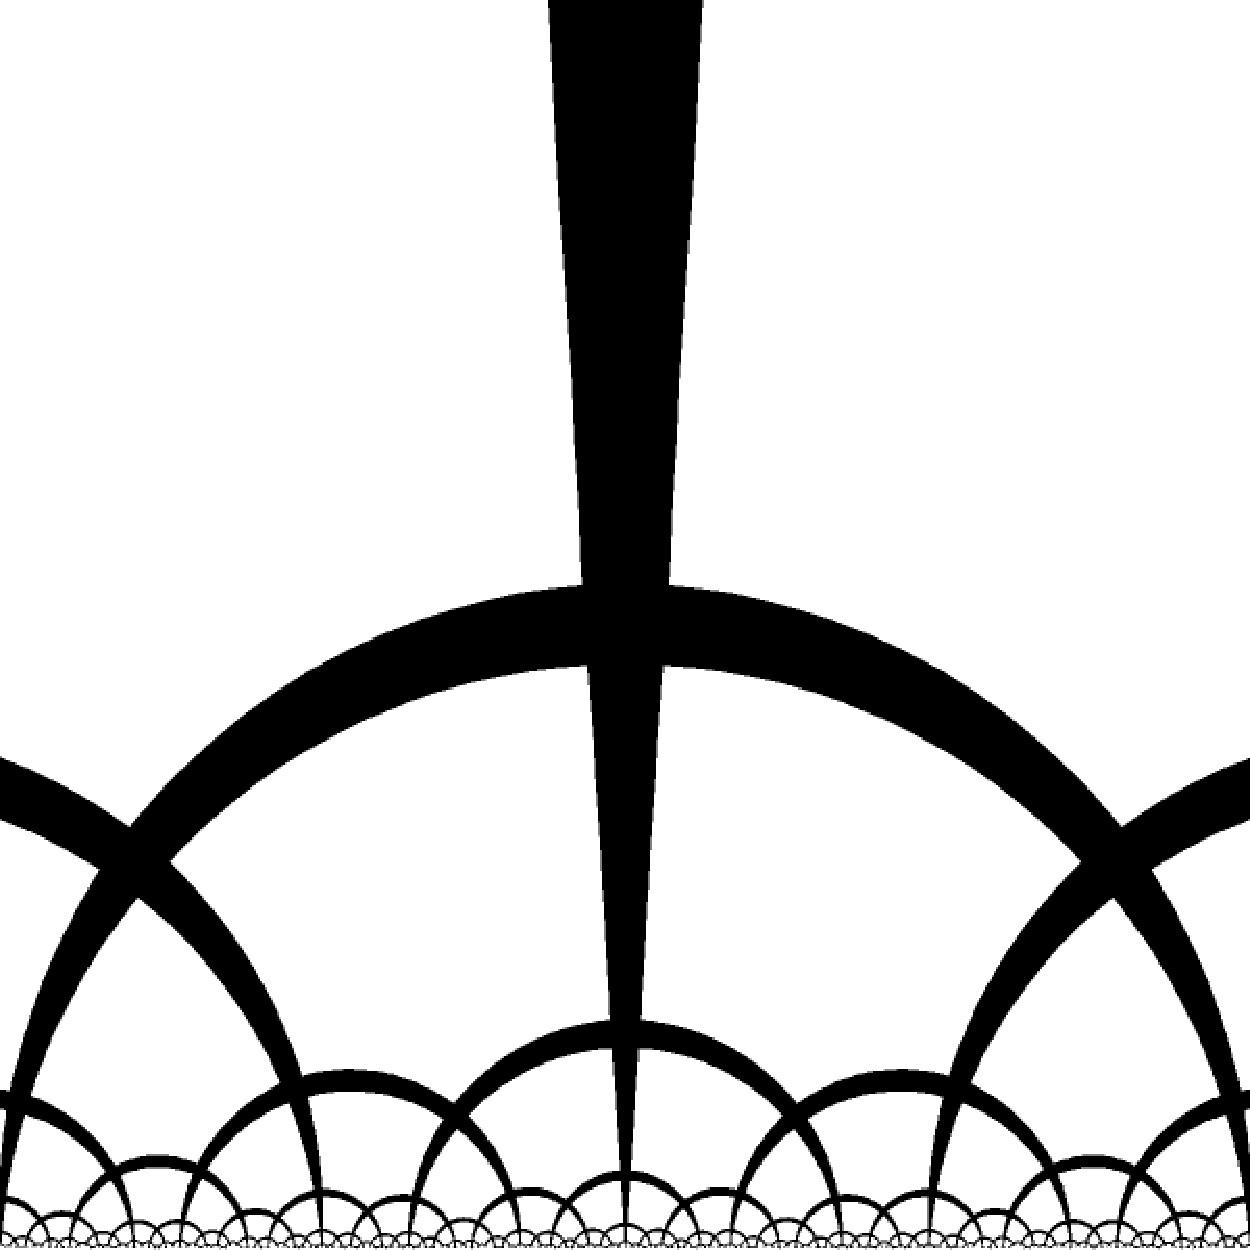
\includegraphics[width=.8 \linewidth]{art/tiling-uhp.pdf}
    \caption{Tiling of the Upper Half-Plane by~\citet{bulatovConformal}. The lines
    are geodesic curves}
\end{wrapfigure}

Obtained from the disk via inversion in the sphere \( S((0, -1), \sqrt{2}) \)
(and similarly in higher dimensions).


Results in underlying set \( \{ x\in\mathbb{R}^n \left|~x_n > 0\right.\} \)
and the pull-back metric \( \frac{1}{x_n^2} \operatorname{d}\mathrm{x} \).
Distance of a vertical segment can be easily integrated...
Geodesic between points on the same vertical line is exactly the vertical line segment...
M\"obius transformations are isometries...
One can move any two points onto same vertical line via M\"obius transformation
and then compute the distance...
Stereographic projection is also a simple M\"obius transformation, specifically
an inversion in a sphere (plus throwing away a coordinate)...

\section{Other models}

A different projection could give the Klein model where geodesics are straight
Euclidean lines. Another interesting projection is the Band model which allows
to make a chosen curve appear as a straight line. Very motivating overviews
are~\citet{bulatovConformal} and everything related to the amazing
\texttt{HyperRogue}~\cite{hyperrogue} project.

\section*{Group of isometries of hyperbolic plane}

We've already mentioned the M\"obius (Lie) group...
Please refer to~\cite{beardonGeometryDiscrete,hubbardTeichmuller}

\section{Tilings}

As \citet{yaSaTilingBased} demonstrated, tilings and discrete groups acting on
Hyperbolic spaces are of utmost importance. An entry point is~\citet{gromov}.


\section{Harmonic analysis}

For our further work on ``hyperbolic convolutions'' we need to gain some
familiarity with Harmonic Analysis and Gauge Theory.
\nameref{sec:equivariant} provides a number of relevant links.
\citet{stollharmonic} discusses PDEs on real Hyperbolic space, and e.g.
describes solutions to Laplace equation (the spherical harmonics).

\section{Barycentres vs Einstein midpoints}

Averaging in metric spaces relates to the notion of a barycentre of a measure:
a point \( b \) of a metric space \( (M, \rho) \) is a barycentre of a measure
\( \mu \) if it minimizes the variance functional
\[ b \mapsto \int \rho(b, \cdot)^2\operatorname{d}\mu. \]

An average or mean of \( n \) points, say \( p_1, \ldots, p_n \), is a
barycentre of the uniform measure concentrated on those points, i.e. barycentre
of \( \frac1n\sum_{i=1}^n \delta_{p_i} \).

The Einstein's midpoint, used e.g. in~\cite{khrulkov} is not
the\footnote{``the'', as in negatively-curved spaces barycentres are unique and
always exist}
variance minimizer for Hyperbolic space. Instead, ``Einstein's midpoint'', or
Einstein's \emph{average} of relativistic velocities \( v_1, \ldots, v_n \)
(relative to a chosen rest frame) of particles with invariant masses \( m_1,
\ldots, m_n \), is the velocity of the center-of-momentum frame of
this system. To give sense of what functional ``midpoint'' minimizes, the
center-of-momentum frame is the frame in which total energy of the system is
minimized, or, equivalently, one in which perceived total momentum vanishes.

\citet{diffThroughFrechet} propose a differentiable iterative algorithm
that computes the true mean. See also \citet{gdFrechetHyperbolic}.
